%%%%%%%%%%%%%%%%%%%%%%%%%%%%%%%%%%%%%%%%%
% Beamer Presentation
% LaTeX Template
% Version 1.0 (10/11/12)
%
% This template has been downloaded from:
% http://www.LaTeXTemplates.com
%
% License:
% CC BY-NC-SA 3.0 (http://creativecommons.org/licenses/by-nc-sa/3.0/)
%
%%%%%%%%%%%%%%%%%%%%%%%%%%%%%%%%%%%%%%%%%

%----------------------------------------------------------------------------------------
%	PACKAGES AND THEMES
%----------------------------------------------------------------------------------------

%\documentclass[usenames,dvipsnames]{beamer}
\documentclass[usenames,dvipsnames,handout]{beamer}

%\documentclass{beamer}

\mode<presentation> {

% The Beamer class comes with a number of default slide themes
% which change the colors and layouts of slides. Below this is a list
% of all the themes, uncomment each in turn to see what they look like.

%\usetheme{default}
%\usetheme{AnnArbor}
%\usetheme{Antibes}
%\usetheme{Bergen}
%\usetheme{Berkeley}
%\usetheme{Berlin}
%\usetheme{Boadilla}
%\usetheme{CambridgeUS}
%\usetheme{Copenhagen}
%\usetheme{Darmstadt}
%\usetheme{Dresden}
%\usetheme{Frankfurt}
%\usetheme{Goettingen}
%\usetheme{Hannover}
%\usetheme{Ilmenau}
%\usetheme{JuanLesPins}
%\usetheme{Luebeck}
\usetheme{Madrid}
%\usetheme{Malmoe}
%\usetheme{Marburg}
%\usetheme{Montpellier}
%\usetheme{PaloAlto}
%\usetheme{Pittsburgh}
%\usetheme{Rochester}
%\usetheme{Singapore}
%\usetheme{Szeged}
%\usetheme{Warsaw}

% As well as themes, the Beamer class has a number of color themes
% for any slide theme. Uncomment each of these in turn to see how it
% changes the colors of your current slide theme.

%\usecolortheme{albatross}
%\usecolortheme{beaver}
%\usecolortheme{beetle}
%\usecolortheme{crane}
%\usecolortheme{dolphin}
%\usecolortheme{dove}
%\usecolortheme{fly}
%\usecolortheme{lily}
%\usecolortheme{orchid}
%\usecolortheme{rose}
%\usecolortheme{seagull}
%\usecolortheme{seahorse}
\usecolortheme{whale}
%\usecolortheme{wolverine}

%\setbeamertemplate{footline} % To remove the footer line in all slides uncomment this line
%\setbeamertemplate{footline}[page number] % To replace the footer line in all slides with a simple slide count uncomment this line

%\setbeamertemplate{navigation symbols}{} % To remove the navigation symbols from the bottom of all slides uncomment this line

%remove the icon
\setbeamertemplate{bibliography item}{\insertbiblabel}

%remove line breaks
\setbeamertemplate{bibliography entry title}{}
\setbeamertemplate{bibliography entry location}{}
\setbeamertemplate{bibliography entry note}{}


}

\usepackage{amsfonts}
\usepackage{amsmath}
\usepackage{amssymb}
\usepackage{subcaption}
\usepackage{mathtools}

\usepackage{graphicx} % Allows including images
%\usepackage{booktabs} % Allows the use of \toprule, \midrule and \bottomrule in tables
%\usepackage{tikz}
%\usetikzlibrary{chains}
%\usetikzlibrary{fit}
%\usepackage{pgflibraryarrows}		%optional
%\usepackage{pgflibrarysnakes}		%optional


%\usepackage[usenames,dvipsnames]{color}


%\usepackage[dvipsnames]{xcolor}

%\usepackage{epsfig}
%\usetikzlibrary{shapes.symbols,patterns} % for source symbols
%\usepackage{pgfplots}


%----------------------------------------------------------------------------------------
%	TITLE PAGE
%----------------------------------------------------------------------------------------

\title[]{Resource theory of asymmetric distinguishability} % The short title appears at the bottom of every slide, the full title is only on the title page

\author{Mark M. Wilde} % Your name
\institute[LSU] % Your institution as it will appear on the bottom of every slide, may be shorthand to save space
{
Hearne Institute for Theoretical Physics,\\
Department of Physics and Astronomy,\\
Center for Computation and Technology,\\
Louisiana State University,\\
Baton Rouge, Louisiana, USA \\ % Your institution for the title page
\medskip
\textit{mwilde@gmail.com}\\ % Your email address
\bigskip
Based on arXiv:1905.11629, arXiv:1907.06306\\
 with Xin Wang (University of Maryland and Baidu, Inc.) \\
\bigskip
\bigskip
%QuILT Day, Louisiana State University, July 19, 2019
}
\date{} % Date, can be changed to a custom date

\begin{document}

\begin{frame}
\titlepage % Print the title page as the first slide
\end{frame}

\begin{frame}
\frametitle{Motivation} % Table of contents slide, comment this block out to remove it
%\tableofcontents % Throughout your presentation, if you choose to use \section{} and \subsection{} commands, these will automatically be printed on this slide as an overview of your presentation


\begin{itemize}
\item<2-> {\color{MidnightBlue}\textbf{Distinguishability}} plays a central role in all sciences
\vspace{.1in}
\item<3-> Repeated trials of an experiment allow for increasing the distinguishability between two different hypotheses
\vspace{.1in}
\item<4-> If the two different hypotheses are relatively distinguishable, then fewer trials are needed
\vspace{.1in}
\item<5-> So distinguishability is a {\color{MidnightBlue}\textbf{resource}} in this sense because it limits the amount of effort needed to make decisions
\vspace{.1in}
\item<6-> Statistical and, more generally, quantum hypothesis testing provide a rigorous setting for studying distinguishability
\end{itemize}

\end{frame}

\begin{frame}
\frametitle{Main message}

\begin{itemize}
\item<2-> Distinguishability is a resource that can be quantified and interconverted ({\color{MidnightBlue}\textbf{resource theory of asymmetric distinguishability}})\\(see also \cite{Mats10,M11} for earlier work)
\vspace{.1in}
\item<3-> Fundamental unit is the {\color{MidnightBlue}\textbf{bit of asymmetric distinguishability}}
\vspace{.1in}
\item<4-> Objects to manipulate include state boxes, channel boxes, and quantum strategy (or comb) boxes, and basic tasks include distillation, dilution, and box transformations
\vspace{.1in}
\item<5-> One-shot tasks give {\color{MidnightBlue}\textbf{operational meaning}} to one-shot relative entropies, like non-smooth and smooth min- and max-relative entropy
\vspace{.1in}
\item<6-> {\color{MidnightBlue}\textbf{Quantum relative entropy}} emerges as  fundamental exchange rate 
\end{itemize}


\end{frame}

\begin{frame}
\frametitle{Resource theory of asymmetric distinguishability}

\begin{itemize}

\pause
\item Basic object to manipulate is a ``{\color{MidnightBlue}\textbf{state box}},'' consisting of two quantum states $\rho$ and $\sigma$:
$$
(\rho, \sigma)
$$

\pause
\vspace{.1in}
\item Interpretation: quantum system  prepared in an unknown state


\end{itemize}

\end{frame}

\begin{frame}
\frametitle{Free operations}

\begin{itemize}
\pause
\item What can you do with a state box?
\pause
\vspace{.1in}
\item Any quantum channel $\mathcal{N}$ is allowed for free

\pause
\vspace{.1in}
\item 
You can then convert one state box to another one as follows:
$$
(\rho, \sigma) \quad \rightarrow \quad (\mathcal{N}(\rho), \mathcal{N}(\sigma))
$$
 
 \pause
 \vspace{.1in}
\item Some channels are {\color{MidnightBlue}\textbf{reversible}}, i.e., isometric channels $\mathcal{U}$ or those that append a common quantum state $\tau$:
$$
(\rho, \sigma) \quad\leftrightarrow\quad (\mathcal{U}(\rho), \mathcal{U}(\sigma)) \quad\leftrightarrow\quad (\rho \otimes \tau, \sigma \otimes \tau)
$$
\end{itemize}

\end{frame}

\begin{frame}

\frametitle{Exact box transformation problem}

\pause
\begin{block}{Fundamental question of the resource theory}

\begin{itemize}

\pause
\item Given state boxes $(\rho, \sigma)$ and  $(\tau, \omega)$, is there a quantum channel $\mathcal{N}$ that takes the state box $(\rho, \sigma)$ to the state box $(\tau, \omega)$?

\pause
\vspace{.1in}
\item Equivalently, is there a quantum channel $\mathcal{N}$ such that 
$$
\mathcal{N}(\rho) = \tau, \qquad \mathcal{N}(\sigma) = \omega   ?
$$
\end{itemize}

\end{block}

\begin{itemize}

\pause
\item This question has a long history both in classical and quantum information theory \cite{B53,AU80,CJW04,MOA11,Buscemi2012,HJRW12,BDS14,BHNOW15,Ren16,BD16,Buscemi2016,GJBDM18,B17,BG17}

\pause
\vspace{.1in}
\item It can be solved by semi-definite programming (efficient algorithm)

\pause
\vspace{.1in}
\item It is also known as {\color{MidnightBlue}\textbf{quantum relative majorization}} \cite{BG17} and some  entropic  characterizations are known

\end{itemize}

\end{frame}

\begin{frame}
\frametitle{Approximate box transformation problem}

\begin{itemize}
\pause
\item 
Performing exact transformations of state boxes can be challenging in experimental scenarios.

\pause
\vspace{.1in}
\item Moreover, if the transformation were performed with small error, this would not be noticeable in practice

%\item This motivates the approximate box transformation problem:

\end{itemize}

\pause
\begin{block}{More fundamental question of the resource theory}

\begin{itemize}

\pause
\item Given state boxes $(\rho, \sigma)$ and  $(\tau, \omega)$, how well can a quantum channel~$\mathcal{N}$  take the state box $(\rho, \sigma)$ to  $(\tau, \omega)$ approximately?

\pause
\vspace{.1in}
\item Specifically, how small can the following error $\varepsilon$ be for some quantum channel $\mathcal{N}$, such that
$$
\mathcal{N}(\rho) \approx_{\varepsilon} \tau, \qquad \text{and} \qquad \mathcal{N}(\sigma) = \omega   \quad ?
$$

\pause
\item Allowing error in conversion of first state but not in second state is why this is the resource theory of {\color{MidnightBlue}\textbf{asymmetric}} distinguishability

\end{itemize}

\end{block}


\end{frame}

\begin{frame}
\frametitle{Approximate box transformation problem (ctd.)}

\begin{itemize}

\pause
\item We quantify error in terms of {\color{MidnightBlue}\textbf{normalized trace distance}}, due to its strong operational meaning in terms of absolute deviation of observable probabilities in any quantum-physical experiment:
$$
\zeta_1 \approx_{\varepsilon} \zeta_2 \qquad \Longleftrightarrow \qquad \frac{1}{2} \left \Vert \zeta_1 - \zeta_2 \right \Vert_1 \leq \varepsilon
$$

\pause
\vspace{.1in}
\item Then approx.~box transformation is the following optimization:
$$
\varepsilon((\rho,\sigma)\rightarrow(\tau,\omega
))\coloneqq \label{eq:approx-box-trans}
\inf_{\mathcal{N}\in\text{CPTP}}\left\{  \varepsilon\in\left[  0,1\right]
:\mathcal{N}(\rho)\approx_{\varepsilon}\tau,\ \mathcal{N}(\sigma
)=\omega\right\}  ,
$$

\pause
\vspace{.1in}
\item This can be written as a semi-definite program:
\begin{align*}
\inf_{Y_{B},J_{RB}^{\mathcal{N}} \geq 0}\left\{
\begin{array}
[c]{c}%
\operatorname{Tr}[Y_{B}]:
Y_{B}\geq\tau_{B}-\operatorname{Tr}_{R}[\rho_{R}^{T}J_{RB}^{\mathcal{N}}],\\
\operatorname{Tr}_{R}[\sigma_{R}^{T}J_{RB}^{\mathcal{N}}]=\omega_{B},\
\operatorname{Tr}_{B}[J_{RB}^{\mathcal{N}}]=I_{R}
\end{array}
\right\}
\end{align*}


\end{itemize}


\end{frame}

\begin{frame}
\frametitle{Asymptotic version of approximate box transformation}

\begin{itemize}

\pause
\item Let's think like Claude Shannon and Charlie Bennett... 

%\pause
%\vspace{.1in}
%\item (How 'bout that Shannon award!!!)

\pause
\vspace{.1in}
\item Let $n,m\in\mathbb{Z}^{+}$ and $\varepsilon\in\left[  0,1\right]
$.

\pause
\vspace{.1in}
\item An $(n,m,\varepsilon)$ box transformation protocol for the boxes
$(\rho,\sigma)$ and $(\tau,\omega)$ consists of a channel $\mathcal{N}^{(n)}$
such that
$$
\mathcal{N}^{(n)}(\rho^{\otimes n})  \approx_{\varepsilon}%
\tau^{\otimes m},\qquad
\mathcal{N}^{(n)}(\sigma^{\otimes n})  =\omega^{\otimes
m}.
$$

\pause
\vspace{.1in}
\item
A rate $R$ is \textit{achievable} if for all $\varepsilon\in(0,1]$,
$\delta>0$, and sufficiently large~$n$, there exists an $(n,n[R-\delta
],\varepsilon)$ box transformation protocol.

\pause
\vspace{.1in}
\item {\color{MidnightBlue}\textbf{Optimal box transformation
rate}} $R((\rho,\sigma)\rightarrow(\tau,\omega))$ is equal to the supremum
of all achievable rates.

\end{itemize}

\end{frame}

\begin{frame}
\frametitle{Solution of asymptotic box transformation problem}

\pause
\begin{block}{Quantum relative entropy is the fundamental exchange rate}
Given state boxes $(\rho,\sigma)$ and $(\tau,\omega)$, the optimal box transformation rate is equal to the ratio of quantum relative entropies:
$$
R((\rho,\sigma)\rightarrow(\tau,\omega)) = \frac{D(\rho\Vert\sigma)}{D(\tau\Vert\omega
)}
$$
where $D(\rho \Vert \sigma) \coloneqq  \operatorname{Tr}[\rho [\log_2 \rho - \log_2 \sigma]]$ \cite{U62}.

\end{block}

\begin{itemize}

\pause
\vspace{.1in}
\item Highlights the fundamental role of quantum relative entropy in the resource theory of asymmetric distinguishability

\pause
\vspace{.1in}
\item Resource theory is {\color{MidnightBlue}\textbf{asymptotically reversible}}

\end{itemize}


\end{frame}


\begin{frame}
\frametitle{Solution of asymptotic box transformation problem (ctd.)}
\begin{itemize}

\pause
\item How to prove this? Inspired by entanglement theory \cite{BBPS96,BDSW96}, break task into two: {\color{MidnightBlue}\textbf{distillation}} and
{\color{MidnightBlue}\textbf{dilution}}

\pause
\vspace{.1in}
\item For distillation, convert $(\rho^{\otimes n},\sigma^{\otimes n})$ to fiducial currency (bits of asymmetric distinguishability), \& for dilution, convert these to $(\tau^{\otimes m},\omega^{\otimes m})$. This is the main idea behind the achievability part.

\pause
\vspace{.1in}
\item For the (strong) converse part, use a {\color{MidnightBlue}\textbf{pseudo-continuity bound}} for sandwiched R\'enyi relative entropy and data processing:
\pause
\begin{block}{Pseudo-continuity bound}
Let $\rho_{0}$, $\rho_{1}$, and
$\sigma$ be states such that $\operatorname{supp}(\rho_{0}%
)\subseteq\operatorname{supp}(\sigma)$. Fix $\alpha\in(1/2,1)$ and
$\beta\equiv\beta(\alpha)\coloneqq \alpha/\left(  2\alpha-1\right)  >1$. Then%
\begin{equation*}
\widetilde{D}_{\beta}(\rho_{0}\Vert\sigma)-\widetilde{D}_{\alpha}(\rho
_{1}\Vert\sigma)\geq\frac{\alpha}{1-\alpha}\log F(\rho_{0},\rho_{1}).
\end{equation*}
\end{block}

\end{itemize}

\end{frame}


\begin{frame}
\frametitle{Bits of asymmetric distinguishability}

\begin{itemize}

\pause
\item Fundamental unit  is the ``{\color{MidnightBlue}\textbf{bit of asymmetric distinguishability}}'':
$$
(|0\rangle\!\langle 0 |, \pi) \qquad \text{ where } \pi = I/2
$$

\pause
\vspace{.1in}
\item {\color{MidnightBlue}\textbf{$m$ bits of asymmetric distinguishability}} are encoded in the box
$$
(|0\rangle\!\langle 0 |^{\otimes m}, \pi^{\otimes m})
$$

\pause
\vspace{.1in}
\item Common quantum channels lead to the following equivalence:
$$
(|0\rangle\!\langle 0 |^{\otimes m}, \pi^{\otimes m}) \qquad \leftrightarrow \qquad  (|0\rangle\!\langle 0 |, \pi_{2^m}),
$$
where $\pi_{2^m} = \frac{1}{2^m}|0\rangle\!\langle 0 | + \left(1-\frac{1}{2^m}\right)  |1\rangle\!\langle 1 |$.



\end{itemize}

\end{frame}

\begin{frame}
\frametitle{Bits of asymmetric distinguishability (ctd.)}

More generally, $\log_2 M $ bits of asymmetric distinguishability are encoded in the following state box:
$$
(|0\rangle\!\langle 0 |, \pi_M)
$$
where $$\pi_{M} \coloneqq  \frac{1}{M}|0\rangle\!\langle 0 | + \left(1-\frac{1}{M}\right)  |1\rangle\!\langle 1 |.$$

\end{frame}


\begin{frame}
\frametitle{Exact distinguishability distillation}

\begin{itemize}

\pause
\item Goal: distill from state box $(\rho,\sigma)$ as many exact bits of AD as possible

\pause
\item That is, we want to perform the conversion:
$$
(\rho,\sigma) \rightarrow (|0\rangle\!\langle 0 |, \pi_M)
$$
with $M$ as large as possible.

\pause
\item Formally, {\color{MidnightBlue}\textbf{one-shot exact distillable distinguishability}}  is given by
$$
D_{d}^{0}(\rho,\sigma)\coloneqq 
\log_{2}\sup_{\mathcal{P}\in\text{CPTP}}\left\{  M:\mathcal{P}(\rho
)=|0\rangle\!\langle0|,\ \mathcal{P}(\sigma)=\pi_{M}\right\}  
$$

\pause
\item Key result: It is equal to the {\color{MidnightBlue}\textbf{min-relative entropy}} of \cite{D09}:
$$
D_{d}^{0}(\rho,\sigma) = D_{\min}(\rho \Vert \sigma)
$$
where $D_{\min}(\rho \Vert \sigma) \coloneqq  -\log_{2}\operatorname{Tr}[\Pi_{\rho}%
\sigma]$

\end{itemize}

\end{frame}


\begin{frame}
\frametitle{Exact distinguishability dilution}

\begin{itemize}

\pause
\item Goal: prepare state box $(\rho,\sigma)$ with as few exact bits of AD as possible

\pause
\item That is, we want to perform the conversion:
$$
(|0\rangle\!\langle 0 |, \pi_M) \rightarrow  (\rho,\sigma) 
$$
with $M$ as small as possible.

\pause
\item Formally, {\color{MidnightBlue}\textbf{one-shot exact distinguishability cost}}  is given by
$$
D_{c}^{0}(\rho,\sigma)\coloneqq 
\log_{2}\inf_{\mathcal{P}\in\text{CPTP}}\left\{  M:\mathcal{P}(|0\rangle
\langle0|)=\rho,\ \mathcal{P}(\pi_{M})=\sigma\right\}  
$$

\pause
\item Key result: It is equal to the {\color{MidnightBlue}\textbf{max-relative entropy}} of \cite{D09}:
$$
D_{c}^{0}(\rho,\sigma)=D_{\max}(\rho\Vert\sigma)
$$
where $D_{\max}(\rho\Vert\sigma)    \coloneqq \inf\left\{  \lambda\geq0:\rho\leq2^{\lambda
}\sigma\right\}$

\end{itemize}

\end{frame}


\begin{frame}
\frametitle{Approximate distinguishability distillation}

\begin{itemize}

\pause
\item Goal: distill from state box $(\rho,\sigma)$ as many approx.~bits of AD as possible

\pause
\item That is, we want to perform the conversion:
$$
(\rho,\sigma) \rightarrow (\widetilde{0}_{\varepsilon}, \pi_M)
$$
with $M$ as large as possible and $\widetilde{0}_{\varepsilon} \approx_{\varepsilon} |0\rangle \langle 0|$.

\pause
\item Formally, {\color{MidnightBlue}\textbf{one-shot distillable distinguishability}}  is given by
$$
D_{d}^{\varepsilon}(\rho,\sigma)\coloneqq 
\log_{2}\sup_{\mathcal{P}\in\text{CPTP}}\left\{  M:\mathcal{P}(\rho
)\approx_{\varepsilon} |0\rangle\!\langle0|,\ \mathcal{P}(\sigma)=\pi_{M}\right\}  
$$

\pause
\item Equal to {\color{MidnightBlue}\textbf{smooth min-relative entropy}} of \cite{BD10,BD11,WR12}:
$$
D_{d}^{\varepsilon}(\rho,\sigma) = D_{\min}^{\varepsilon}(\rho \Vert \sigma)
$$
where $D_{\min}^{\varepsilon}(\rho \Vert \sigma) \coloneqq  -\log_{2}\inf_{\Lambda \geq 0}\{ \operatorname{Tr}[\Lambda%
\sigma] : \Lambda\leq I , \operatorname{Tr}[\Lambda \rho]\geq 1- \varepsilon\}$

\end{itemize}

\end{frame}


\begin{frame}
\frametitle{Approximate distinguishability dilution}

\begin{itemize}

\pause
\item Goal: prepare state box $(\rho,\sigma)$ approximately using as few bits of AD as possible

\pause
\item That is, we want to perform the conversion:
$$
(|0\rangle\!\langle 0 |, \pi_M) \rightarrow  (\widetilde{\rho},\sigma) 
$$
with $M$ as small as possible and $\widetilde{\rho} \approx_{\varepsilon} \rho$.

\pause
\item Formally, {\color{MidnightBlue}\textbf{one-shot distinguishability cost}}  is given by
$$
D_{c}^{\varepsilon}(\rho,\sigma)\coloneqq 
\log_{2}\inf_{\mathcal{P}\in\text{CPTP}}\left\{  M:\mathcal{P}(|0\rangle
\langle0|)\approx_{\varepsilon}\rho,\ \mathcal{P}(\pi_{M})=\sigma\right\}  
$$

\pause
\item Key result: It is equal to {\color{MidnightBlue}\textbf{smooth max-relative entropy}} of \cite{D09}:
$$
D_{c}^{\varepsilon}(\rho,\sigma)=D_{\max}^{\varepsilon}(\rho\Vert\sigma)
$$
where $D_{\max}^{\varepsilon}(\rho\Vert\sigma)    \coloneqq \inf_{\widetilde{\rho} \approx_{\varepsilon} \rho}D_{\max}(\widetilde{\rho} \Vert \sigma)$.

\end{itemize}

\end{frame}


\begin{frame}
\frametitle{Asymptotics}

\begin{itemize}

\pause
\item {\color{MidnightBlue}\textbf{Asymptotic distillable distinguishability}}:
$$
D_{d}(\rho,\sigma)  \coloneqq  \lim_{\varepsilon \to 0} \lim_{n \to \infty}\frac{1}{n}D_{d}^{\varepsilon}(\rho^{\otimes n},\sigma^{\otimes n}) 
  = D(\rho \Vert \sigma)
$$
Last equality follows from quantum Stein's lemma \cite{HP91} (refinements available in \cite{ON00,N06,Hay07,tomamichel2013hierarchy,li14,MO13})

\pause
\item {\color{MidnightBlue}\textbf{Asymptotic distinguishability cost}}:
$$
D_{c}(\rho,\sigma)  \coloneqq  \lim_{\varepsilon \to 0} \lim_{n \to \infty}\frac{1}{n}D_{c}^{\varepsilon}(\rho^{\otimes n},\sigma^{\otimes n}) 
 = D(\rho \Vert \sigma)
$$
Last equality follows from asymptotic equipartition property \cite{TCR09} (refinements available in \cite{tomamichel2013hierarchy}). Open questions about error and strong converse exponents

\pause
\item Resource theory is {\color{MidnightBlue}\textbf{asymptotically reversible}}

\end{itemize}

\end{frame}


\begin{frame}
\frametitle{Resource theory for channels}

\begin{itemize}

\pause
\item We can generalize the resource theory of asymmetric distinguishability to {\color{MidnightBlue}\textbf{quantum channels}}

\vspace{.1in}

\pause
\item The basic object to manipulate is a {\color{MidnightBlue}\textbf{channel box}}, consisting of two channels $\mathcal{N}$ and $\mathcal{M}$:
$$
(\mathcal{N},\mathcal{M})
$$

\pause
\vspace{.1in}
\item Quantum channel boxes have inputs and outputs, and so the ways that we can manipulate them are richer than for state boxes

\pause
\vspace{.1in}
\item Tasks for the state theory have generalizations to the channel theory (distillation, dilution, channel box transformations)

\end{itemize}

\end{frame}


\begin{frame}
\frametitle{Free operations are quantum superchannels}

\begin{itemize}

\pause
\item Most general physical transformation of a quantum channel is  a {\color{MidnightBlue}\textbf{superchannel}} \cite{CDP08}, which accepts as input a quantum channel and outputs a quantum channel

\pause
\vspace{.2in}
\item The superchannel $\Theta_{\left(  A\rightarrow B\right)
\rightarrow\left(  C\rightarrow D\right)  }$ takes as input a quantum channel
$\mathcal{N}_{A\rightarrow B}$ and outputs a quantum channel $\mathcal{K}%
_{C\rightarrow D}$, which we denote by%
$$
\Theta_{\left(  A\rightarrow B\right)  \rightarrow\left(  C\rightarrow
D\right)  }(\mathcal{N}_{A\rightarrow B})=\mathcal{K}_{C\rightarrow D}.
$$

\end{itemize}

\end{frame}

\begin{frame}
\frametitle{Physical realizations of quantum superchannels}

\begin{itemize}

\pause
\item Superchannel has a {\color{MidnightBlue}\textbf{physical realization}} in terms of 
pre- and post-processing quantum channels \cite{CDP08} (see also \cite{G18}):
$$
\Theta_{\left(  A\rightarrow B\right)  \rightarrow\left(  C\rightarrow
D\right)  }(\mathcal{N}_{A\rightarrow B})
=\mathcal{D}_{BM\rightarrow D}\circ\mathcal{N}_{A\rightarrow B}\circ
\mathcal{E}_{C\rightarrow AM},
$$
where $\mathcal{E}_{C\rightarrow AM}$ and $\mathcal{D}_{BM\rightarrow D}$ are
pre- and post-processing  channels

\end{itemize}

\pause
\begin{figure}[ptb]
\begin{center}
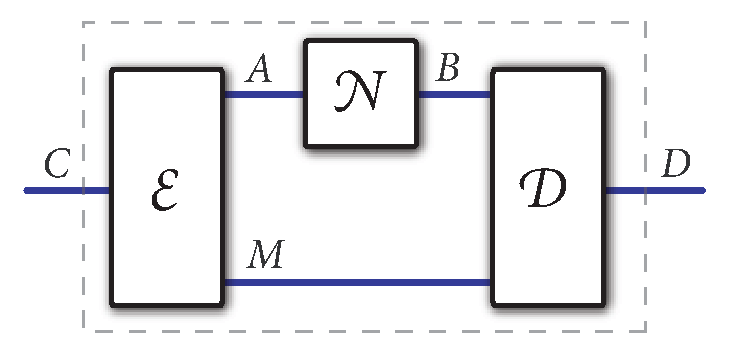
\includegraphics[
width=0.8\linewidth
]{superchannel.pdf}
\end{center}
\end{figure}


\end{frame}

\begin{frame}
\frametitle{Exact channel box transformation problem}

\begin{block}{Fundamental question of the resource theory \cite{G18}}

\begin{itemize}

\pause
\item Given channel boxes $(\mathcal{N}, \mathcal{M})$ and $(\mathcal{K}, \mathcal{L})$, is there a quantum superchannel $\Theta$ that takes the channel box
$(\mathcal{N}, \mathcal{M})$ to the channel box $(\mathcal{K},  \mathcal{L})$?

\pause
\vspace{.1in}
\item Specifically, is there a quantum superchannel $\Theta$ such that 
$$
\Theta(\mathcal{N}) = \mathcal{K}, \qquad \Theta(\mathcal{M}) = \mathcal{L}   ?
$$

\end{itemize}

\end{block}

\begin{itemize}

\pause
\vspace{.1in}
\item This was called ``comparison of channels'' in \cite{G18}

\pause
\vspace{.1in}
\item \cite{G18} showed that it can be solved by means of a semi-definite program and characterized by the extended conditional min-entropy

\end{itemize}

\end{frame}


\begin{frame}
\frametitle{Approximate channel box transformation problem}

\begin{block}{Fundamental question of the resource theory}

\begin{itemize}

\pause
\item Given channel boxes $(\mathcal{N}, \mathcal{M})$ and  $(\mathcal{K}, \mathcal{L})$, how well can a quantum superchannel $\Theta$ take the channel box
$(\mathcal{N}, \mathcal{M})$ to the channel box $(\mathcal{K},  \mathcal{L})$ approximately?

\pause
\vspace{.1in}
\item Specifically, how small can the following error $\varepsilon$ be for some superchannel $\Theta$ such that 
$$
\Theta(\mathcal{N}) \approx_{\varepsilon} \mathcal{K}, \qquad \text{and} \qquad \Theta(\mathcal{M}) = \mathcal{L}   \qquad ?
$$




\end{itemize}

\end{block}

\end{frame}


\begin{frame}
\frametitle{Approximate channel box transformation problem (ctd.)}

\begin{itemize}

\pause
\item Quantify error in terms of {\color{MidnightBlue}\textbf{normalized diamond distance}} \cite{Kitaev1997}, due to its strong operational meaning in terms of absolute deviation of observable probabilities in any quantum-physical experiment:
$$
\mathcal{N}_1 \approx_{\varepsilon} \mathcal{N}_2 \qquad \Longleftrightarrow \qquad \frac{1}{2} \left \Vert \mathcal{N}_1 - \mathcal{N}_2 \right \Vert_{\diamond} \leq \varepsilon
$$

\pause
\vspace{.1in}
\item Then approx.~channel box transformation is the optimization
$$
\varepsilon((\mathcal{N},\mathcal{M})\rightarrow(\mathcal{K},\mathcal{L}
))\coloneqq 
\inf_{\Theta\in\text{SC}}\left\{  \varepsilon\in\left[  0,1\right]
:\Theta(\mathcal{N})\approx_{\varepsilon}\mathcal{K},\ \Theta(\mathcal{M})=\mathcal{L}\right\}  ,
$$

\pause
\vspace{.1in}
\item This can be written as a semi-definite program:
\begin{equation*}
\inf_{Z_{CD},\ \Gamma_{CBAD}^{\Theta}\geq0}\left\Vert \operatorname{Tr}%
_{D}[Z_{CD}]\right\Vert _{\infty}, \label{eq:SDP-primal-box-tr-1} \text{ subject to }
\end{equation*}
\begin{align*}
Z_{CD}  &  \geq\Gamma_{CD}^{\mathcal{K}}-\operatorname{Tr}_{AB}[(\Gamma
_{AB}^{\mathcal{N}})^{T}\Gamma_{CBAD}^{\Theta}],\quad 
\Gamma_{CD}^{\mathcal{L}}    =\operatorname{Tr}_{AB}[(\Gamma_{AB}%
^{\mathcal{M}})^{T}\Gamma_{CBAD}^{\Theta}],\nonumber\\
\Gamma_{CB}^{\Theta}  &  =I_{CB},\quad
\Gamma_{CBA}^{\Theta}    =\Gamma_{CA}^{\Theta}\otimes\pi_{B},
\label{eq:SDP-primal-box-tr-2}%
\end{align*}


\end{itemize}


\end{frame}

\begin{frame}
\frametitle{Asymptotic parallel  channel box transformation}

\begin{itemize}

\pause
\item Again think like Claude Shannon and Charlie Bennett...

\pause
\vspace{.1in}
\item Let $n,m\in\mathbb{Z}^{+}$ and $\varepsilon\in\left[  0,1\right]
$.

\pause
\vspace{.1in}
\item An $(n,m,\varepsilon)$ {\color{MidnightBlue}\textbf{parallel channel box transformation protocol}} for the channel boxes
$(\mathcal{N},\mathcal{M})$ and $(\mathcal{K},\mathcal{L})$ consists of a superchannel $\Theta^{(n)}$
such that
$$
\Theta^{(n)}(\mathcal{N}^{\otimes n}) \approx_{\varepsilon}%
\mathcal{K}^{\otimes m},\qquad
\Theta^{(n)}(\mathcal{M}^{\otimes n})=\mathcal{L}^{\otimes
m}.
$$

\pause
\vspace{.1in}
\item
A rate $R$ is \textit{achievable} if for all $\varepsilon\in(0,1]$,
$\delta>0$, and sufficiently large~$n$, there exists an $(n,n[R-\delta
],\varepsilon)$ parallel channel box transformation protocol.

\pause
\vspace{.1in}
\item {\color{MidnightBlue}\textbf{Optimal parallel channel box transformation}}
rate $R^p((\mathcal{N},\mathcal{M})\rightarrow(\mathcal{K},\mathcal{L}))$ is equal to supremum
of all achievable rates.

\end{itemize}

\end{frame}

\begin{frame}
\frametitle{Partial solution}

\pause
Solution for classical--quantum and environment-seizable \cite{BHKW18} channels in terms of {\color{MidnightBlue}\textbf{channel relative entropy}} \cite{Cooney2016,LKDW18}

\pause
\begin{block}{Quantum relative entropy is the fundamental exchange rate}
Given classical--quantum or environment-seizable channel boxes $(\mathcal{N},\mathcal{M})$ and $(\mathcal{K},\mathcal{L})$, the optimal parallel channel box transformation rate is equal to the ratio of channel relative entropies:
$$
R^p((\mathcal{N},\mathcal{M})\rightarrow(\mathcal{K},\mathcal{L})) = \frac{D(\mathcal{N}\Vert\mathcal{M})}{D(\mathcal{K}\Vert\mathcal{L}
)}
$$
where $D(\mathcal{N} \Vert \mathcal{M}) \coloneqq  \sup_{\psi_{RA}} D(\mathcal{N}_{A \to B} (\psi_{RA}) \Vert \mathcal{M}_{A\to B}(\psi_{RA}))$ \cite{Cooney2016,LKDW18}.

\end{block}

\begin{itemize}


\pause

\vspace{.1in}
\item (Parallel) resource theory asymptotically reversible for these channels

\end{itemize}


\end{frame}


\begin{frame}
\frametitle{Partial solution (ctd.)}
\begin{itemize}

\pause
\item How to prove this? Again break task into two: distillation and dilution

\pause
\vspace{.1in}
\item For distillation, convert $(\mathcal{N}^{\otimes n},\mathcal{M}^{\otimes n})$ to bits of asymmetric distinguishability, \& for dilution, convert these to $(\mathcal{K}^{\otimes m},\mathcal{L}^{\otimes m})$. This solves achievability part for special channels.

\pause
\vspace{.1in}
\item For the (strong) converse part, use a pseudo-continuity bound for sandwiched R\'enyi relative entropy and data processing:
\pause
\begin{block}{Pseudo-continuity bound}
Let $\mathcal{N}_{A\rightarrow
B}^{0}$, $\mathcal{N}_{A\rightarrow B}^{1}$, and $\mathcal{M}_{A\rightarrow
B}$ be channels such that $D_{\max}(\mathcal{N}^{0}\Vert\mathcal{M})<\infty$.
Then for $\alpha\in(1/2,1)$ and $\beta\coloneqq \alpha/\left(
2\alpha-1\right)  >1$, 
\begin{equation*}
\widetilde{D}_{\beta}(\mathcal{N}^{0}\Vert\mathcal{M})-\widetilde{D}_{\alpha
}(\mathcal{N}^{1}\Vert\mathcal{M})\geq\frac{\alpha}{1-\alpha}\log
_{2}F(\mathcal{N}^{0},\mathcal{N}^{1}).
\end{equation*}
\end{block}

\end{itemize}

\end{frame}


\begin{frame}
\frametitle{Bits of asymmetric distinguishability}

\begin{itemize}

\pause
\item Identify $\log_2 M $ bits of asymmetric distinguishability as follows:
$$
(|0\rangle\!\langle 0 |, \pi_M) \quad \leftrightarrow \quad (\mathcal{R}^{|0\rangle\!\langle 0 |}, \mathcal{R}^{\pi_M})
$$
where $$\pi_{M} \coloneqq  \frac{1}{M}|0\rangle\!\langle 0 | + \left(1-\frac{1}{M}\right)  |1\rangle\!\langle 1 |$$ and $\mathcal{R}^{\sigma}(\rho) = \operatorname{Tr}[\rho]\sigma$ is a replacer channel that replaces the input state $\rho$ with the state $\sigma$


\end{itemize}

\end{frame}



\begin{frame}
\frametitle{Exact distinguishability distillation}

\begin{itemize}

\pause
\item Goal: distill from  box $(\mathcal{N},\mathcal{M})$ as many exact bits of AD as possible

\pause
\item That is, we want to perform the conversion:
$$
(\mathcal{N},\mathcal{M}) \rightarrow (\mathcal{R}^{|0\rangle\!\langle 0 |}, \mathcal{R}^{\pi_M})
$$
with $M$ as large as possible.

\pause
\item Formally, {\color{MidnightBlue}\textbf{one-shot exact distillable distinguishability}}  is given by
$$
D_{d}^{0}(\mathcal{N},\mathcal{M})\coloneqq 
\log_{2}\sup_{\Theta\in\text{SC}}\left\{  M:
\Theta(\mathcal{N}
)=\mathcal{R}^{|0\rangle\!\langle 0 |},\ \Theta(\mathcal{M})=\mathcal{R}^{\pi_M}\right\}  
$$

\pause
\item Key result: It is equal to the {\color{MidnightBlue}\textbf{channel min-relative entropy}}:
$$
D_{d}^{0}(\mathcal{N},\mathcal{M}) = D_{\min}(\mathcal{N}  \Vert\mathcal{M})
$$
where $D_{\min}(\mathcal{N}  \Vert\mathcal{M}) \coloneqq  \sup_{\psi_{RA}} D_{\min}(\mathcal{N}_{A \to B} (\psi_{RA}) \Vert \mathcal{M}_{A\to B}(\psi_{RA}))$.

\end{itemize}

\end{frame}


\begin{frame}
\frametitle{Exact distinguishability dilution}

\begin{itemize}

\pause
\item Goal: prepare channel box $(\mathcal{N},\mathcal{M})$ with as few exact bits of AD as possible

\pause
\item That is, we want to perform the conversion:
$$
(\mathcal{R}^{|0\rangle\!\langle 0 |}, \mathcal{R}^{\pi_M}) \rightarrow (\mathcal{N},\mathcal{M})
$$
with $M$ as small as possible.

\pause
\item Formally, {\color{MidnightBlue}\textbf{one-shot exact distinguishability cost}}  is given by
$$
D_{c}^{0}(\mathcal{N},\mathcal{M})\coloneqq 
\log_{2}\inf_{\Theta\in\text{SC}}\left\{  M:
\mathcal{N}
=\Theta(\mathcal{R}^{|0\rangle\!\langle 0 |}),\ \mathcal{M}=\Theta(\mathcal{R}^{\pi_M})\right\}
$$

\pause
\item = {\color{MidnightBlue}\textbf{channel max-relative entropy}} \cite{Cooney2016,LKDW18,GFWRSCW18}
$$
D_{c}^{0}(\mathcal{N},\mathcal{M})=D_{\max}(\mathcal{N}  \Vert\mathcal{M})
$$
where $D_{\max}(\mathcal{N}  \Vert\mathcal{M})    \coloneqq \sup_{\psi_{RA}} D_{\max}(\mathcal{N}_{A \to B} (\psi_{RA}) \Vert \mathcal{M}_{A\to B}(\psi_{RA}))$

\end{itemize}

\end{frame}


\begin{frame}
\frametitle{Approximate distinguishability distillation}

\begin{itemize}

\pause
\item Goal: distill from box $(\mathcal{N},\mathcal{M})$ as many approx.~bits of AD as possible

\pause
\item That is, we want to perform the conversion:
$$
(\mathcal{N},\mathcal{M}) \rightarrow (\widetilde{\mathcal{R}}^{|0\rangle\!\langle 0 |}, \mathcal{R}^{\pi_M})
$$
with $M$ as large as possible and $\widetilde{\mathcal{R}}^{|0\rangle\!\langle 0 |} \approx_{\varepsilon} \mathcal{R}^{|0\rangle\!\langle 0 |}$.

\pause
\item Formally, {\color{MidnightBlue}\textbf{one-shot distillable distinguishability}}  is given by
$$
D_{d}^{\varepsilon}(\mathcal{N}  ,\mathcal{M})\coloneqq 
\log_{2}\sup_{\Theta\in\text{SC}}\left\{  M:
\Theta(\mathcal{N}
)\approx_{\varepsilon}\mathcal{R}^{|0\rangle\!\langle 0 |},\ \Theta(\mathcal{M})=\mathcal{R}^{\pi_M}\right\}  
$$

\pause
\item Equal to {\color{MidnightBlue}\textbf{smooth channel min-relative entropy}} of \cite{Cooney2016}:
$$
D_{d}^{\varepsilon}(\mathcal{N}  ,\mathcal{M}) = D_{\min}^{\varepsilon}(\mathcal{N}  \Vert\mathcal{M})
$$
where $D_{\min}^{\varepsilon}(\mathcal{N}  \Vert\mathcal{M}) \coloneqq  \sup_{\psi_{RA}} D_{\min}^{\varepsilon}(\mathcal{N}_{A \to B} (\psi_{RA}) \Vert \mathcal{M}_{A\to B}(\psi_{RA}))$

\end{itemize}

\end{frame}


\begin{frame}
\frametitle{Approximate distinguishability dilution}

\begin{itemize}

\pause
\item Goal: prepare box $(\mathcal{N}  ,\mathcal{M})$ approximately using as few bits of AD as possible

\pause
\item That is, we want to perform the conversion:
$$
(\mathcal{R}^{|0\rangle\!\langle 0 |}, \mathcal{R}^{\pi_M}) \rightarrow  (\widetilde{\mathcal{N}}  ,\mathcal{M}) 
$$
with $M$ as small as possible and $\widetilde{\mathcal{N}} \approx_{\varepsilon} \mathcal{N}$.

\pause
\item Formally, {\color{MidnightBlue}\textbf{one-shot distinguishability cost}}  is given by
$$
D_{c}^{\varepsilon}(\mathcal{N},\mathcal{M})\coloneqq 
\log_{2}\inf_{\Theta\in\text{SC}}\left\{  M:
\mathcal{N}
\approx_{\varepsilon} \Theta(\mathcal{R}^{|0\rangle\!\langle 0 |}),\ \mathcal{M}=\Theta(\mathcal{R}^{\pi_M})\right\}
$$

\pause
\item Equal to {\color{MidnightBlue}\textbf{smooth channel max-relative entropy}} of \cite{GFWRSCW18}:
$$
D_{c}^{\varepsilon}(\mathcal{N},\mathcal{M})=D_{\max}^{\varepsilon}(\mathcal{N}\Vert\mathcal{M})
$$
where $D_{\max}^{\varepsilon}(\mathcal{N}\Vert\mathcal{M})    \coloneqq \inf_{\widetilde{\mathcal{N}} \approx_{\varepsilon} \mathcal{N}}D_{\max}(\widetilde{\mathcal{N}} \Vert \mathcal{M})$.

\end{itemize}

\end{frame}


\begin{frame}
\frametitle{Asymptotics (parallel case)}

\begin{itemize}

\pause
\item {\color{MidnightBlue}\textbf{Asymptotic parallel distillable distinguishability}}:
$$
D_{d}(\mathcal{N},\mathcal{M})  \coloneqq  \lim_{\varepsilon \to 0} \lim_{n \to \infty}\frac{1}{n}D_{d}^{\varepsilon}(\mathcal{N}^{\otimes n},\mathcal{M}^{\otimes n}) 
  = \lim_{m \to \infty} \frac{1}{m}D(\mathcal{N} \Vert \mathcal{M})
$$
Follows essentially from quantum Stein's lemma \cite{HP91} and converse bounds for $D_{\min}^{\varepsilon}$ \cite{WR12,MW12,KW17}

\pause
\item {\color{MidnightBlue}\textbf{Asymptotic parallel distinguishability cost}}:
$$
D_{c}(\rho,\sigma)  \coloneqq  \lim_{\varepsilon \to 0} \lim_{n \to \infty}\frac{1}{n}D_{c}^{\varepsilon}(\mathcal{N}^{\otimes n},\mathcal{M}^{\otimes n}) 
 \geq \lim_{m \to \infty} \frac{1}{m}D(\mathcal{N} \Vert \mathcal{M})
$$
Last equality is operational (cost $\geq$ distillability). Whether equality holds is related to open question of \cite{LW19}

\pause
\item Resource theory is asymptotically reversible for classical--quantum and environment-seizable channel boxes

\end{itemize}

\end{frame}


\begin{frame}
\frametitle{Sequential setting}


\pause
\begin{block}{$(n,m,\varepsilon)$ sequential channel box transformation protocol}
Goal is to convert $n$-round sequential channel box $(\mathcal{N}^{(n)},\mathcal{M}^{(n)})$ to $m$-round sequential channel box 
$(\mathcal{K}^{(m)},\mathcal{L}^{(m)})$ by means of a physical transformation $\Theta^{(n\to m)}$ (quantum strategy \cite{GW07} or comb \cite{CDP09}), such that 
$$\Theta^{(n\to m)}(\mathcal{N}^{(n)}) \approx_{\varepsilon} \mathcal{K}^{(m)}, \qquad \Theta^{(n\to m)} (\mathcal{M}^{(n)})= \mathcal{L}^{(m)}$$
\end{block}



\end{frame}


\begin{frame}
\frametitle{Depiction of condition $\Theta^{(n\to m)}(\mathcal{N}^{(n)}) \approx_{\varepsilon} \mathcal{K}^{(m)}$}

\begin{figure}[ptb]
\begin{center}
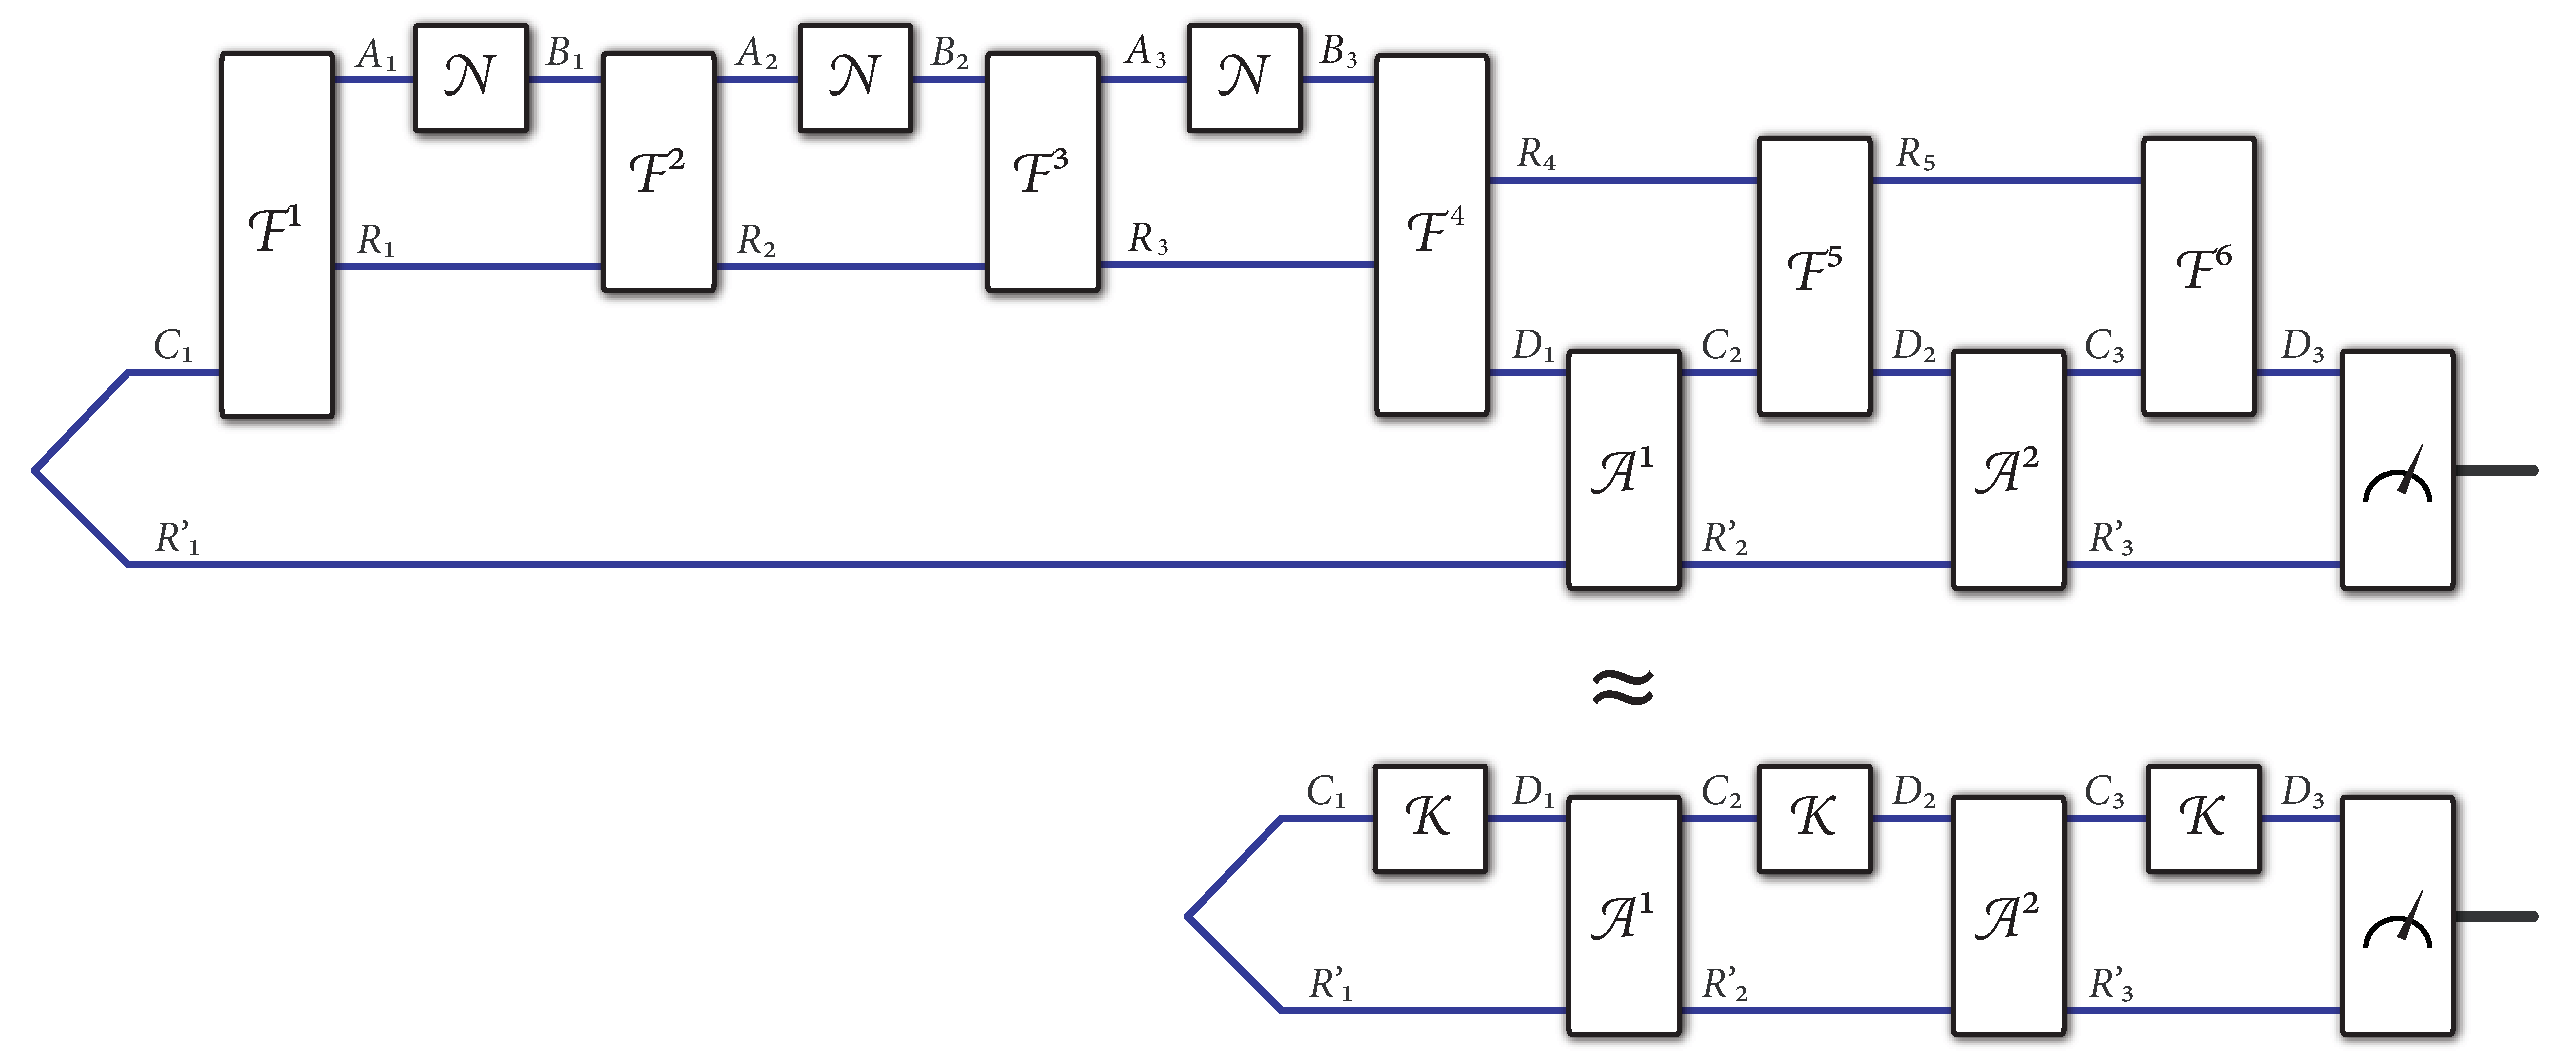
\includegraphics[
width=\linewidth
]
{sequential-ch-box-trans.pdf}
\end{center}
\end{figure}

Observable probabilities between $\Theta^{(n\to m)}(\mathcal{N}^{(n)})$ and $\mathcal{K}^{(m)}$ deviate by no more than $\varepsilon$ when paired up with an arbitrary co-strategy \cite{GW07} or tester~\cite{CDP09} (operational definition of {\color{MidnightBlue}\textbf{strategy distance}} \cite{GW07,CDP09})

\end{frame}

\begin{frame}
\frametitle{Depiction of condition $\Theta^{(n\to m)} (\mathcal{M}^{(n)})= \mathcal{L}^{(m)}$}

\begin{figure}[ptb]
\begin{center}
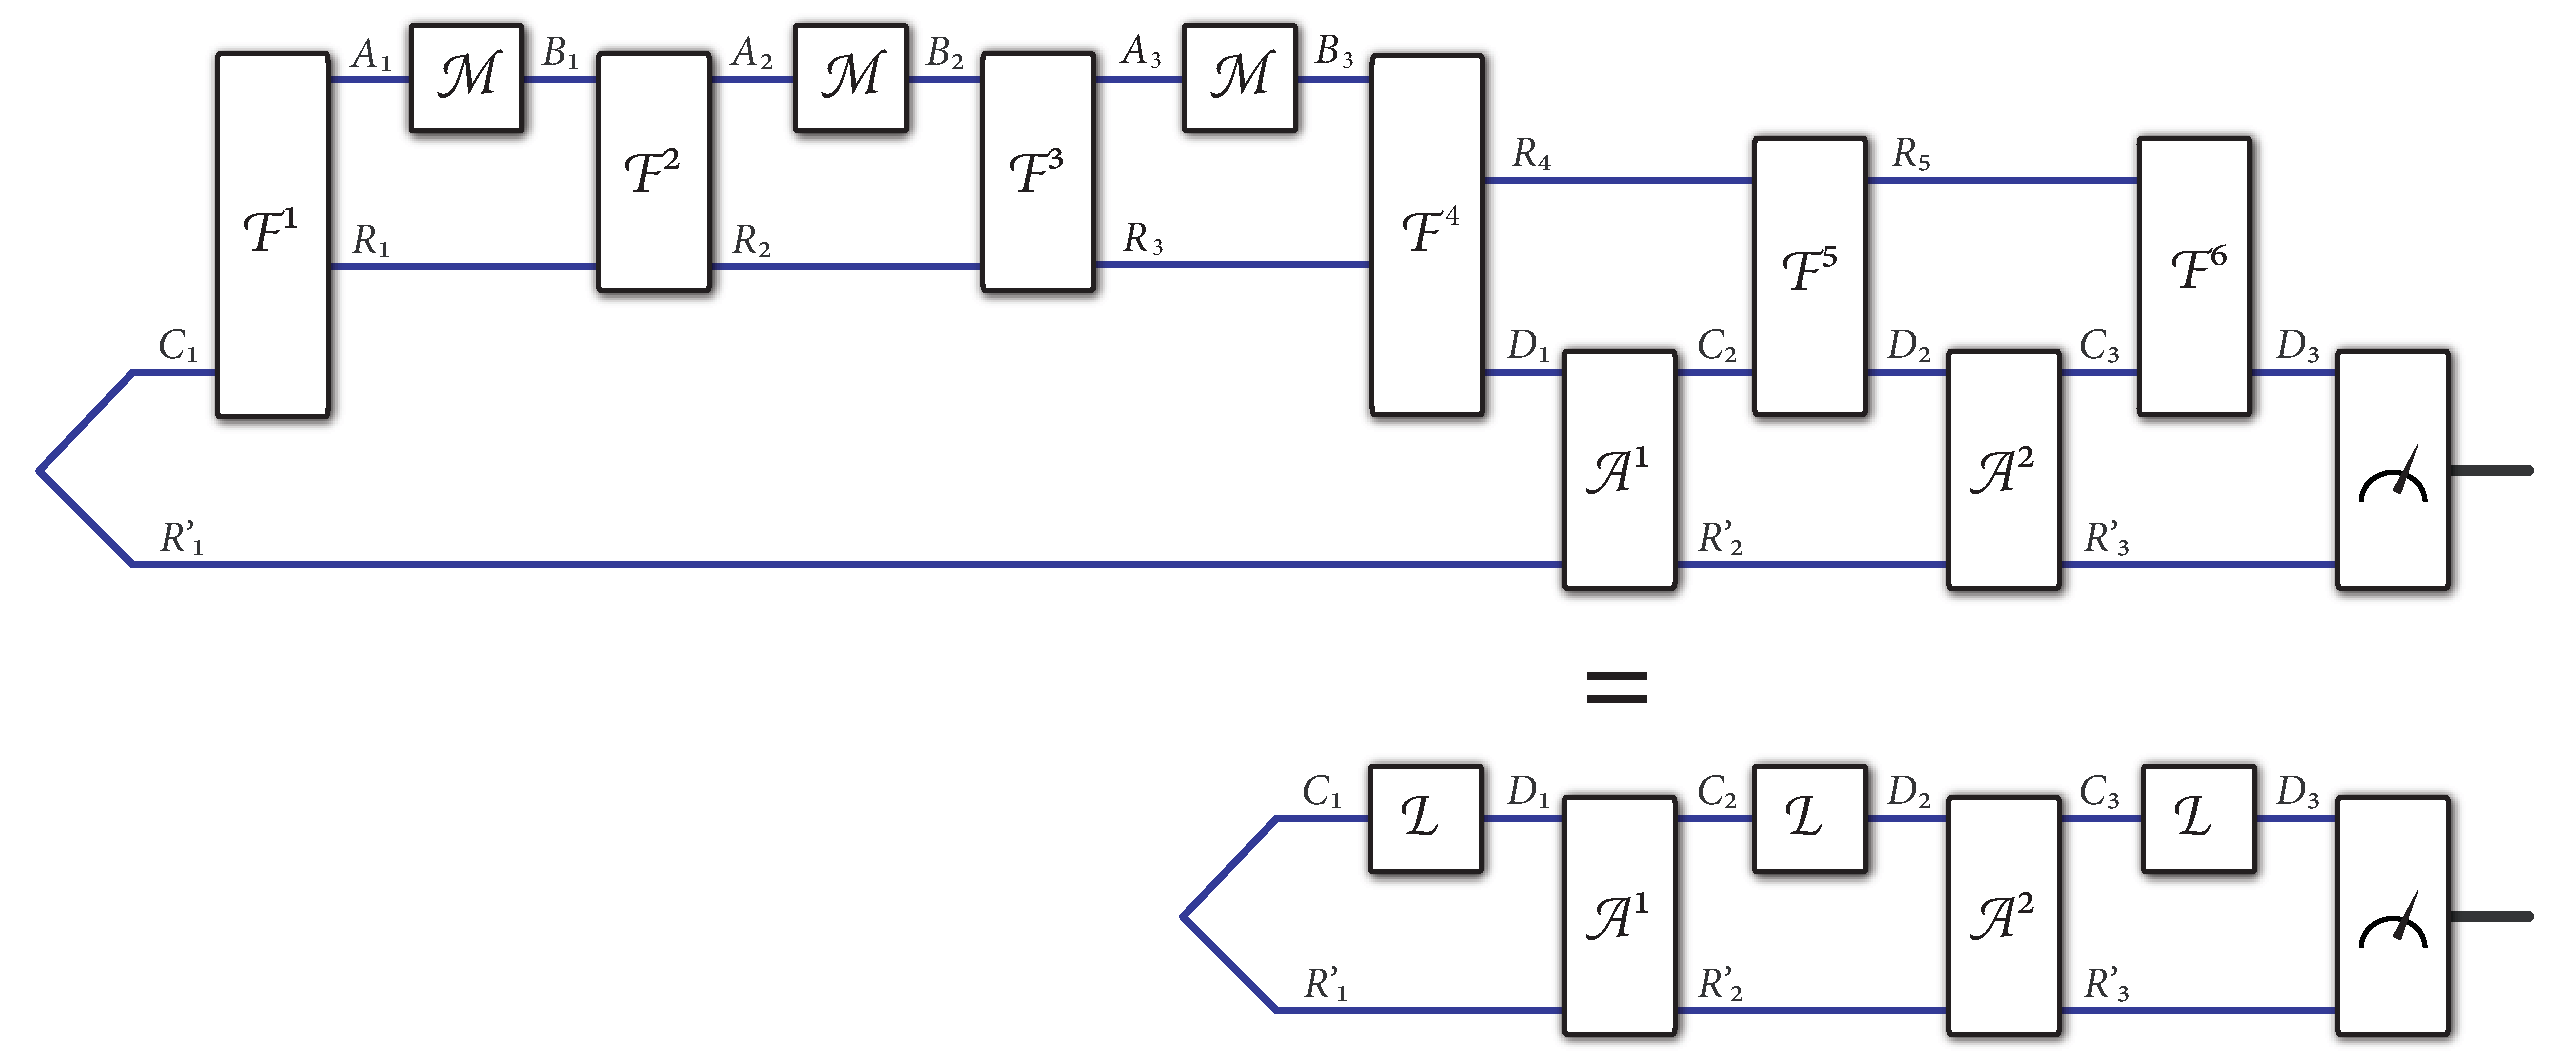
\includegraphics[
width=\linewidth
]
{sequential-ch-box-trans-2.pdf}
\end{center}
\end{figure}

Observable probabilities between $\Theta^{(n\to m)}(\mathcal{N}^{(n)})$ and $\mathcal{K}^{(m)}$ do not deviate at all when paired up w/ an arbitrary co-strategy \cite{GW07} or tester~\cite{CDP09} (equivalent to Choi states being equal \cite{GW07,CDP09})

\end{frame}





\begin{frame}
\frametitle{Exact sequential distinguishability dilution}


\begin{itemize}

\pause
\item Goal: Prepare sequential channel box $(\mathcal{N}^{(n)},\mathcal{M}^{(n)})$ with as few bits of AD as possible

\pause
\item Formally, {\color{MidnightBlue}\textbf{exact distinguishability cost}} is given by
\begin{multline*}
D_{c}^{0}(\mathcal{N}^{(n)},\mathcal{M}^{(n)})\coloneqq 
\inf_{\Theta^{(1\rightarrow n)}}\left\{
\begin{array}
[c]{c}%
\log_{2}M:\mathcal{N}^{(n)} = \Theta^{(1\rightarrow n)}(\mathcal{R}%
_{C\rightarrow D}^{|0\rangle\!\langle0|}),\\
\mathcal{M}^{(n)} =\Theta^{(1\rightarrow n)}(\mathcal{R}_{C\rightarrow D}%
^{\pi_{M}})
\end{array}
\right\}  .
\end{multline*}

\pause
\item Key result: Using ``bootstrapping'' method of \cite{GFWRSCW18}, normalized cost equal to channel max-relative entropy for all $n\geq 1$:
$$
\frac{1}{n} D_{c}^{0}(\mathcal{N}^{(n)},\mathcal{M}^{(n)}) = D_{\max}(\mathcal{N}\Vert\mathcal{M})
$$

\pause
\item Implies that asymptotic exact sequential cost is
$$
D_{c}^{0}(\mathcal{N},\mathcal{M}) \coloneqq  \lim_{n \to \infty}\frac{1}{n} D_{c}^{0}(\mathcal{N}^{(n)},\mathcal{M}^{(n)}) = D_{\max}(\mathcal{N}\Vert\mathcal{M})
$$

\end{itemize}


\end{frame}

\begin{frame}
\frametitle{Approximate distinguishability distillation}

\begin{itemize}

\pause
\item Goal: Distill from sequential channel box $(\mathcal{N}^{(n)},\mathcal{M}^{(n)})$ as many approx.~bits of AD as possible

\pause
\item Formally, {\color{MidnightBlue}\textbf{approx.~distillable distinguishability}} is given by
\begin{multline*}
D_{d}^{\varepsilon}(\mathcal{N}^{(n)},\mathcal{M}^{(n)})\coloneqq 
\sup_{\Theta^{(n\rightarrow 1)}}\left\{
\begin{array}
[c]{c}%
\log_{2}M:\Theta^{(n\rightarrow1)}(\mathcal{N}^{(n)}) \approx_{\varepsilon}\mathcal{R}%
_{C\rightarrow D}^{|0\rangle\!\langle0|},\\
\Theta^{(n\rightarrow1)}(\mathcal{M}^{(n)})=\mathcal{R}_{C\rightarrow D}%
^{\pi_{M}}%
\end{array}
\right\}  .
\end{multline*}

\pause
\item Key result: Using a different ``bootstrapping'' method of \cite{GFWRSCW18}, asymptotic sequential distillable distinguishability equal to amortized channel relative entropy of \cite{BHKW18}:
\begin{align*}
D_{d}(\mathcal{N},\mathcal{M}) & \coloneqq  \lim_{\varepsilon \to 0}\lim_{n \to \infty}\frac{1}{n} D_{d}^{\varepsilon}(\mathcal{N}^{(n)},\mathcal{M}^{(n)}) = D_{\mathcal{A}}(\mathcal{N}\Vert\mathcal{M}), \text{ with }\\
D_{\mathcal{A}}(\mathcal{N}\Vert\mathcal{M}) & \coloneqq 
\sup_{\rho_{RA}, \sigma_{RA}} D(\mathcal{N}_{A\to B}(\rho_{RA})\Vert \mathcal{M}_{A \to B}(\sigma_{RA})) - 
D(\rho_{RA}\Vert \sigma_{RA})
\end{align*}

\pause
\item Can also be understood as solution of Stein's lemma for quantum channels in sequential setting

\end{itemize}

\end{frame}


\begin{frame}
\frametitle{Conclusion and future directions}

\begin{itemize}
\pause
\item Resource theory of asymmetric distinguishability developed for states, channels, and even strategies/combs (see arXiv:1907.06306 for details of strategies/combs)

\pause
\vspace{.2in}
\item Some open questions about error and strong converse exponents, second-order expansions, etc.

%\vspace{.2in}
%\pause
%\item Interesting open question: Is there a channel box $(\mathcal{N},\mathcal{M})$ such that
%$$
%D_{\mathcal{A}}(\mathcal{N}\Vert\mathcal{M}) > 
%\lim_{m \to \infty}\frac{1}{m}D(\mathcal{N}^{\otimes m} \Vert \mathcal{M}^{\otimes m})  \quad ?
%$$
%If so, the implication is that a sequential strategy can strictly outperform a parallel strategy in asymmetric quantum channel discrimination. Alternatively, is there equality above for all channels?

\end{itemize}

\end{frame}


%\begin{frame}
%\frametitle{}
%
%\end{frame}
%
%
%\begin{frame}
%\frametitle{}
%
%\end{frame}
%
%
%\begin{frame}
%\frametitle{}
%
%\end{frame}
%
%
%
%\begin{frame}
%\frametitle{}
%
%\end{frame}
%
%
%\begin{frame}
%\frametitle{}
%
%\end{frame}
%
%\begin{frame}
%\frametitle{}
%
%\end{frame}
%
%
%\begin{frame}
%\frametitle{}
%
%\end{frame}
%
%
%\begin{frame}
%\frametitle{}
%
%\end{frame}
%
%\begin{frame}
%\frametitle{}
%
%\end{frame}
%
%
%\begin{frame}
%\frametitle{}
%
%\end{frame}
%
%
%\begin{frame}
%\frametitle{}
%
%\end{frame}
%
%
%\begin{frame}
%\frametitle{}
%
%\end{frame}


%----------------------------------------------------------------------------------------
%	PRESENTATION SLIDES
%----------------------------------------------------------------------------------------

%------------------------------------------------
%\section{First Section} % Sections can be created in order to organize your presentation into discrete blocks, all sections and subsections are automatically printed in the table of contents as an overview of the talk
%------------------------------------------------

%\subsection{Subsection Example} % A subsection can be created just before a set of slides with a common theme to further break down your presentation into chunks

%------------------------------------------------




\begin{frame}[allowframebreaks] %in case more than 1 slide needed
\frametitle{References}
    {\footnotesize
\bibliography{Ref}
\bibliographystyle{alpha}
    }
\end{frame}

%------------------------------------------------

%\begin{frame}
%\Huge{\centerline{The End}}
%\end{frame}

%----------------------------------------------------------------------------------------

\end{document} 